% !TEX root = ../ApproxDA-TransUNet.tex
\section{Method}
\label{sec:method}

This section introduces the overall architecture of ApproxDA-TransUNet and the placement of ApproxDABlocks within it, then details the three independently controllable approximation axes each block implements, and finally analyzes their computational complexity.

\subsection{Architecture Overview}

Figure~\ref{fig:framework} illustrates the overall architecture: ApproxDA-TransUNet adopts the hybrid CNN--ViT encoder-decoder structure of DA-TransUNet~\cite{sun2024datransunet}, with an R50-ViT-B/16 backbone pretrained on ImageNet-21K. Three CNN encoder stages produce multi-scale features at strides 4, 8, and 16; a 12-layer ViT processes $14{\times}14$ patch tokens. ApproxDABlocks replace all dual-attention modules at three skip connections---512 channels at $28{\times}28$, 256 at $56{\times}56$, and 64 at $112{\times}112$---and at the bottleneck. Each block routes activations through a Low-Rank Windowed PAM branch and a Grouped CAM branch, fused by a configurable gate $g$. Figure~\ref{fig:approxda_block} details the internal structure of each ApproxDABlock and its three independently controllable approximation axes.

\begin{figure*}[tbp]
  \centering
  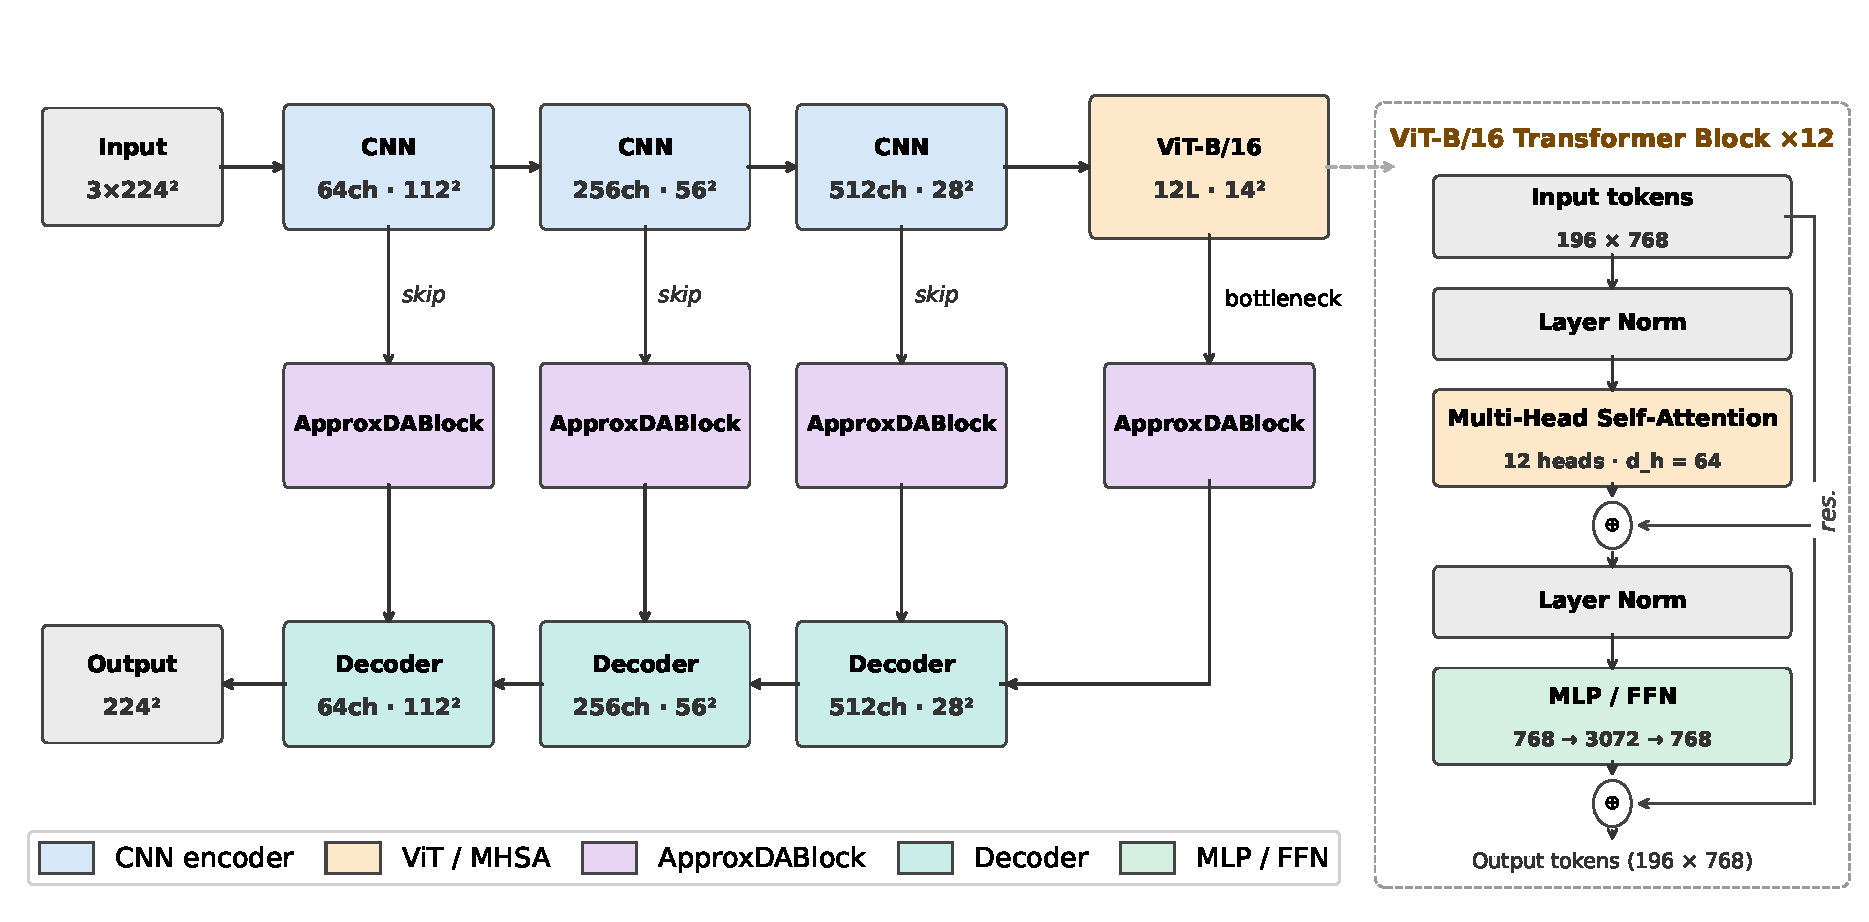
\includegraphics[width=\textwidth]{figures/approxda_overview}
  \caption{ApproxDA-TransUNet overall architecture. ApproxDABlocks replace standard dual-attention modules across all skip connections and the bottleneck.}
  \label{fig:framework}
\end{figure*}

\begin{figure*}[tbp]
  \centering
  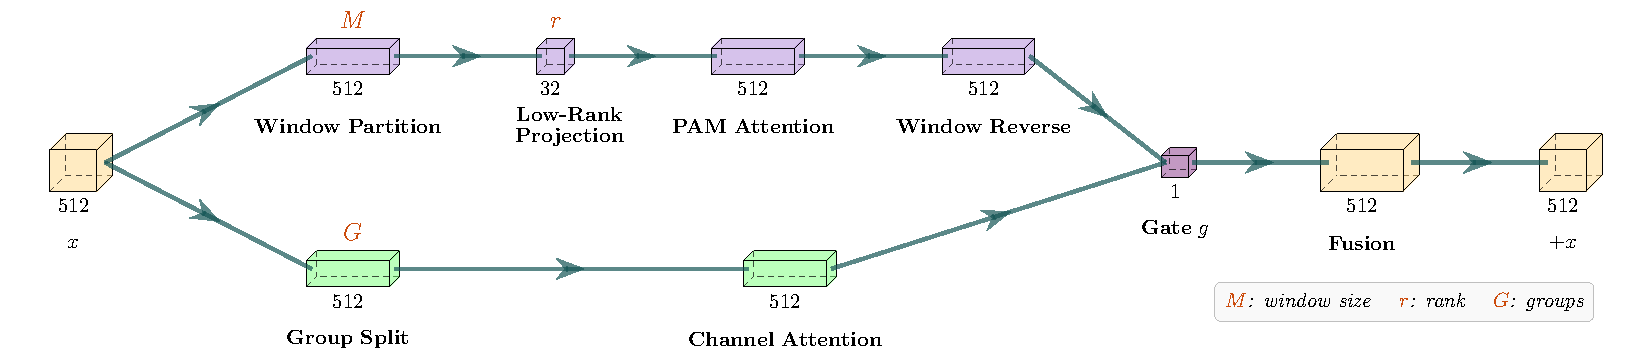
\includegraphics[width=\textwidth]{figures/approxda_block}
  \caption{ApproxDABlock internal structure with three independent approximation axes: spatial scope ($M$), projection rank ($r$), and channel grouping ($G$). Input $\mathbf{x}$ splits into a Low-Rank Windowed PAM branch and a Grouped CAM branch fused by gate $g$.}
  \label{fig:approxda_block}
\end{figure*}

\subsection{Attention Approximation Formulation}

The original DA module performs dense spatial and channel attention over the full feature map, with quadratic complexity in both spatial resolution and channel dimension. ApproxDA-TransUNet reduces this cost along three independent axes, each targeting a distinct aspect of the approximation:

\textbf{Spatial scope} (window size $M$) controls \emph{how far} PAM reaches. Full global attention ($M{=}H$) captures all long-range spatial relationships; restricting to $M{\times}M$ local windows trades long-range context for lower complexity. This axis most directly governs whether tasks with broader contextual requirements retain the anatomical context they depend on.

\textbf{Representation fidelity} (rank $r$) controls \emph{how precisely} attention is computed within each window. Low-rank projection ($r \ll M^2$) approximates the affinity matrix at reduced cost; higher $r$ approaches exact attention.

\textbf{Channel interaction} (groups $G$) controls \emph{which channels} may interact in CAM. Partitioning $C$ channels into $G$ independent groups limits cross-channel dependency to within-group interactions, reducing the interaction scope.

The axes are architecturally independent: any two of $\{M,\,r,\,G\}$ can be held fixed while the third varies. In this paper, $M$ is the axis we systematically ablate (Section~\ref{sec:approx_scale}); gate routing is studied as a separate mechanism (Section~\ref{sec:collapse}); rank $r$ and groups $G$ are exposed as configurable capabilities of the framework, with their held-fixed default values ($r{=}32$, $G{=}8$) used throughout the main results.

\subsection{Spatial Approximation}

Instead of computing global position attention, ApproxDA-TransUNet partitions the feature map into non-overlapping windows of size $M{\times}M$. Attention is computed independently inside each local window, reducing complexity from $\mathcal{O}(N^2C)$ to $\mathcal{O}(NM^2C)$.

\textbf{Window partitioning.} Following~\cite{liu2021swin}, we partition the feature map into $n_W$ non-overlapping $M{\times}M$ windows. Window clamping $M \leftarrow \min(M, H, W)$ allows $M{=}112$ to yield global attention at all scales, enabling a clean ablation that isolates windowing from low-rank as the performance bottleneck.

\textbf{Low-rank projection.} Following~\cite{wang2020linformer}, we compute query, key, and value feature matrices within each window via $1{\times}1$ convolutions, $\mathbf{Q}, \mathbf{K}, \mathbf{V} \in \mathbb{R}^{N_w \times C}$ where $N_w{=}M^2$. A shared learned projection $\mathbf{E} \in \mathbb{R}^{r \times N_w}$ ($r \ll N_w$) reduces the sequence length of the key and value:
\begin{equation}
  \mathbf{K}' = \mathbf{E}\mathbf{K}, \quad \mathbf{V}' = \mathbf{E}\mathbf{V} \in \mathbb{R}^{r \times C}.
  \label{eq:lowrank}
\end{equation}
Attention logits are computed between the full-length query and the rank-$r$ projected key, normalized, and applied to the projected value:
\begin{equation}
  \mathrm{Attn}(\mathbf{Q},\mathbf{K},\mathbf{V}) = \mathrm{softmax}\!\left(\mathbf{Q}\mathbf{K}'^\top\right)\mathbf{V}' \in \mathbb{R}^{N_w \times C},
  \label{eq:lowrank_attn}
\end{equation}
followed by a learnable residual scale, $\mathbf{y} = \alpha \cdot \mathrm{Attn}(\mathbf{Q},\mathbf{K},\mathbf{V}) + \mathbf{x}$, with scalar $\alpha$ initialized to zero (matching our implementation, no $1/\sqrt{C}$ temperature scaling is applied to the logits). Projecting $\mathbf{K}$ and $\mathbf{V}$ costs $\mathcal{O}(N_w r C)$; computing $\mathbf{Q}\mathbf{K}'^\top$ and its product with $\mathbf{V}'$ each cost $\mathcal{O}(N_w r C)$, avoiding the $\mathcal{O}(N_w^2 C)$ cost of full in-window attention. Summed over $N/N_w$ windows, total attention complexity is $\mathcal{O}(NrC)$. Combined, windowing and low-rank projection reduce the theoretical attention-matrix size from $\mathcal{O}(N^2)$ to $\mathcal{O}(Nr)$, a factor of $N/r$ (${\sim}390{\times}$ at $112{\times}112$ with $r{=}32$); note this is a memory/FLOP-count reduction in the attention operation specifically; end-to-end model GFLOPs also include the projection cost $\mathcal{O}(N_wrC)$ and the surrounding convolutional layers, which do not shrink at the same rate (Table~\ref{tab:efficiency}). Window size $M$ forms the primary experimental axis investigated in this study, while rank $r{=}32$ is held fixed in the clean window ablations (Section~\ref{sec:approx_scale}).

\subsection{Channel Approximation}

The original Channel Attention Module computes a $C{\times}C$ channel attention matrix at $\mathcal{O}(C^2N)$ cost. ApproxDA-TransUNet approximates this by partitioning $C$ channels into $G$ groups of width $C_g = C/G$, computing independent per-group attention:
\begin{equation}
  X^{(g)}_{ji} = \frac{\exp(\mathbf{A}^{(g)}_i \cdot \mathbf{A}^{(g)}_j)}{\sum_{k=1}^{C_g}\exp(\mathbf{A}^{(g)}_k \cdot \mathbf{A}^{(g)}_j)},
  \label{eq:groupedcam}
\end{equation}
with total cost $\mathcal{O}(C^2N/G)$. Compared with dense channel interaction, grouped attention significantly reduces computational complexity while preserving local channel dependencies.

The grouping number $G$ provides another controllable approximation dimension, allowing the influence of channel approximation to be studied independently from spatial approximation.

\subsection{Routing Strategy}

The routing of DA-TransUNet~\cite{sun2024datransunet} is extended to a configurable \texttt{gate\_mode}. PAM and CAM outputs are fused via:
\begin{equation}
  \mathbf{y} = \mathbf{W}_f\!\left(g \cdot \hat{\mathbf{P}} + (1-g) \cdot \hat{\mathbf{C}}\right) + \mathbf{x},
  \label{eq:fusion}
\end{equation}
where $\hat{\mathbf{P}}$ and $\hat{\mathbf{C}}$ are the normalized PAM and CAM outputs, $\mathbf{W}_f$ is a $1{\times}1$ convolution, and $g$ is determined by the \texttt{gate\_mode} parameter:

\begin{center}
\small
\begin{tabular}{@{}ll@{}}
\texttt{pam}:   & $g = 1.0$ \quad (PAM only) \\
\texttt{cam}:   & $g = 0.0$ \quad (CAM only) \\
\texttt{fixed}: & $g = 0.5$ \quad (equal blend) \\
\texttt{learn}: & $g = \sigma(\mathbf{W}_g \cdot \mathrm{GAP}(\mathbf{x})) \in (0,1)^C$ \\
\end{tabular}
\end{center}

In gate=learn, $g \in (0,1)^C$ is a per-channel routing coefficient broadcast over all spatial positions; it collapses to a channel-wise blend rather than a spatially-adaptive or input-dependent scalar. This single-parameter design enables systematic ablation of routing strategy without any other architectural change. ApproxDA-TransUNet does not treat this routing module as a primary architectural contribution; rather, it serves as an analyzable component whose optimization dynamics---including an unexpected convergence to $g{\approx}0.5$ regardless of window size---are investigated in Section~\ref{sec:collapse}.

The network is trained with a combined Dice and cross-entropy objective with equal weights:
\begin{equation}
  \mathcal{L} = \tfrac{1}{2}\mathcal{L}_{\text{Dice}} + \tfrac{1}{2}\mathcal{L}_{\text{CE}},
  \label{eq:loss}
\end{equation}
following DA-TransUNet~\cite{sun2024datransunet} for direct comparability. Dice loss optimizes the overlap metric used at evaluation and handles class imbalance naturally; cross-entropy provides stable per-pixel gradient signal throughout training.

